\chapter{Introduzione}

\section{Concetti fondamentali di Ingegneria del Software}
    In questo corso ci occuperemo di sviluppare skill che vanno oltre la programmazione e che servono a sviluppare e manutenere un sistema software.
    Questo processo, e di conseguenza il corso, si dividerà nelle seguenti sezioni:
    \begin{itemize}
        \item M1: Concetti generali dell'ingegneria del software
        \item M2: Analisi e specifica dei requisiti
        \item M3: Progettazione architetturale e ad alto livello: System Design
        \item M4: Progettazione a basso livello: Object Design
        \item M5: Software Testing
    \end{itemize}
    
    \paragraph{Definizione di Software} Secondo lo standard IEEE, il software è l'insieme di programmi, procedure e documentazione compresi in un sistema computerizzato.

    \paragraph{Storia del Software}Nel corso dei decenni il Software ha subito una evoluzione significativa.
    Dapprima esso era \textbf{arte}, ossia prodotto da una singola persona o piccolo gruppo di persone per utilizzo privato.
    
    Poi è diventato \textbf{artigianato}, ossia applicazioni sviluppate da produttori specializzati su richiesta specifica di un cliente.
    
    Infine, esso è divenuto \textbf{industriale}, ossia prodotto per un mercato più o meno grande che sia. Ciò ha causato un grande aumento di complessità, dimensioni e richiesta.
    
\subsection{Programma vs Prodotto}
    Non sono da confondere \textbf{programma} e \textbf{prodotto software}.
    
    In un programma, l'autore è anche il fruitore, mentre in un prodotto software no. Le conseguenze di ciò sono una necessità di documentazione e un approccio più formale al prodotto, in quanto questo avrà dimensioni maggiori e sarà destinato a un pubblico più generale.
    
    Inoltre, la manutenzione di un prodotto software prende il significato di espansione, cambiamento, evoluzione, mentre in un prodotto hardware ciò non è possibile, in quanto la fase successiva al rilascio consiste di poche modifiche e perlopiù riparazioni.
    
    Il prodotto software si suddivide a sua volta in:
    \begin{itemize}
        \item Prodotti generici: Sistemi stand alone da distribuire su un mercato più o meno grande, ma comunque generale. Ciò che l'utente paga è una licenza d'uso, e non il prodotto stesso.
        \item Prodotti specifici: Sistemi commissionati da un fruitore o macrosistema specifico. Il fruitore compra il software nel suo insieme, e non solo una licenza o permesso d'uso.
    \end{itemize}
    
    %----------
    
\section{Principi dell'Ingegneria del Software}
    
\subsection{I principi}
    L'Ingegneria del Software si basa su alcuni importanti principi, quali:
    \begin{itemize}
        \item \textbf{Rigore:} Precisione di progettazione ed esecuzione
        \item \textbf{Formalità:} Più specifica del rigore, è fondamento matematico
        \item \textbf{Separazione di aspetti diversi:} Affrontare in fasi e modi diversi aspetti diversi di un problema più complesso
        \item \textbf{Modularità:} Suddivisione di un sistema complesso in parti più semplici. È importante mantenere un certo livello di indipendenza fra i moduli. Si distingue dalla separazione di cui sopra per l'accezione più pratica
        \item \textbf{Astrazione:} Si identificano gli aspetti cruciali di un determinato problema in un determinato momento, ignorando quelli superflui. Questo garantisce un certo grado di generalizzazione che idealmente dovrebbe essere massimizzato pur mantenendo una descrizione corretta del problema
        \item \textbf{Anticipazione del cambiamento:} Previsione dei cambiamenti a cui il sistema sarà soggetto. Se eseguito bene, il sistema potrà cambiare, crescere ed evolversi senza modificare la sua struttura fondamentale e senza generare ulteriori difetti
        \item \textbf{Generalità:} Tentare di risolvere il problema nella sua accezione più generale. Se eseguito correttamente ha come effetto collaterale l'anticipazione del cambiamento
        \item \textbf{Incrementalità:} Lavorare a un sistema complesso per passi successivi, dando priorità alle core funcionalities e sviluppando solo dopo i dettagli o funzionalità secondarie
        \item \textbf{Metodo (o Tecnica):} Strumento generale per risolvere determinate classi di problemi
        \item \textbf{Metodologia:} Insieme di principi, metodi ed elementi disciplinari che garantiscono l'efficacia del proprio procedere. È più generico del metodo e difatti lo contiene
        \item \textbf{Strumento (Tool):} Strumento per fare qualcosa in modo più preciso, corretto o immediato. È strettamente legato a skill tecniche e le complementa. Alcuni esempi di strumenti sono una IDE, uno strumento di creazione UML, \LaTeX, etc
        \item \textbf{Procedura:} Una combinazione di \textit{strumenti} e \textit{metodi}, più dettagliato di un metodo, descrive precisamente la risoluzione di un problema
        \item \textbf{Paradigma:} Ancora più generale di una \textit{metodologia}, è una filosofia o approccio a un qualcosa
    \end{itemize}
        
\subsection{Processo Software}
    Il processo software può essere formale, semi-formale o informale, ed è definito come l'insieme di organizzato di attività che sovrintendono alla costruzione del prodotto, e comprende \textit{metodi}, \textit{tecniche}, \textit{metodologie} e \textit{strumenti}.
    
    Inoltre è suddiviso in fasi secondo uno schema di riferimento che chiamiamo \textbf{ciclo di vita del software}.
    
    \paragraph{Definizione} Il ciclo di vita del software (CVS) è il periodo che va dal concepimento del prodotto software al momento in cui lo stesso non è più mantenuto. Il modello del CVS è una caratterizzazione descrittiva o prescrittiva (in base a chi lo legge, se persona familiare o nuovo contributore) di come deve essere sviluppato.

\subsection{Fasi del CVS}
    Le fasi generali di molti CVS sono:
    \begin{itemize}
        \item \textbf{Studio di fattibilità:} Serve a valutare se il progetto è fattibile, realistico e quali sono i suoi benefici
        \item \textbf{Analisi dei requisiti:} Analisi più specifica dei bisogni dell'utente, del da farsi e degli standard qualitativi. Il linguaggio usato è comprensibile dall'utente e comunque ad alto livello
        \item \textbf{Progettazione:} Scomposizione del sistema in moduli (architectural design) e specifica dei dettagli interni di ogni componente (detailed design). È in questa fase che si smette di chiedersi il \textbf{cosa} e si inizia a chiedersi il \textbf{come}
        \item \textbf{Programmazione e test di unità:} Codifica di ogni modulo e test dello stesso in isolamento
        \item \textbf{Integrazione e test di sistema:} Integrazione dei moduli e test del sistema nel suo insieme
        \item \textbf{Deployment:} Fase di distribuzione del Software all'utenza
        \item \textbf{Manutenzione:} Fase successiva al rilascio, di evoluzione e cambiamento del Software
    \end{itemize}

\subsection{Modelli di Ciclo di Vita del Software (CVS)}
    \subsubsection{Modello a cascata (Waterfall)}
        Era un modello popolare negli anni '70, avente un approccio ingegneristico derivante dall'industria manifatturiera. Prevedeva la progettazione, la produzione di un prototipo e la messa in produzione.
        
        I suoi \textbf{pro} sono stati la definizione di concetti utili successivamente utilizzati ed espansi in altri modelli, la semplicità di gestione del progetto e la facilità di comprensione del modello stesso.
        
        I suoi \textbf{contro} invece sono stati la mancanza di interazione con il cliente, data dalla struttura modulare ma poco interconnessa delle fasi (una volta conclusa la progettazione difficilmente si modificava il progetto, e una volta mandato in produzione il prodotto difficilmente si tornava a rivedere il prototipo). Il cliente era al corrente di ciò che succedeva solo all'inizio e alla fine dell'intero progetto, la parte intermedia era determinata dalla correttezza di questa interazione iniziale e del progetto.
        
    \subsubsection{V\&V e Retroazione (Feedback)}
        Ci sono stati molti modelli che si basavano sulla struttura di quello a cascata ma al contempo si proponevano di correggere alcuni suoi errori. Per esempio il modello \textbf{V\&V e Retroazione (Feedback)} prevede un controllo alla fine di ogni fase. La natura di questo controllo può essere di diversi tipi (verification, validation o entrambi), e se uno o più di questi controlli falliscono, si torna al passo precedente per rivederlo.
        
        La \textbf{verification (o verifica)} è la valutazione della verità della corrispondenza fra il prodotto e la sua specifica, mentre la \textbf{validation (o convalida)} consta dell'appropriatezza di un prodotto rispetto alla sua missione operativa.
        
        In pratica la verifica testa se ciò che è stato fatto sia corretto, mentre la convalida testa se si è fatta la cosa giusta in primo luogo.
        
        Il concetto di feedback può essere generalizzato, ed esso può far ritorno a una fase precedente arbitraria, e non necessariamente a quella immediatamente precedente.
        
    \subsubsection{Sviluppo evolutivo}
        Questo tipologia di sviluppo del software prevede la rivisitazione di fasi precedenti, anche molto precedenti, del progetto quando necessario. Un approccio del genere accomoda ottimamente il cambiamento dei requisiti e del progetto in corso d'opera, al contrario del modello a cascata, ma si rischia di perdere di vista il progetto nel suo insieme. Inoltre il prodotto potrebbe non avere una struttura solida, e dal punto di vista manageriale la gestione è complessa.
        
    \subsubsection{Trasformazioni formali}
        In questo modello di sviluppo, ogni passo è composto da descrizioni formali e può dare origine in modo quasi automatico al successivo. Un metodo del genere raramente è applicabile in contesti reali, ma può essere utile per lo sviluppo di sistemi critici come per esempio quelli orientati alla safety.
        
    \subsubsection{Sviluppo a componenti}
        Si basa sullo sviluppo e utilizzo di componenti già esistenti (off the shelf). Utile per sistemi sufficientemente generici, ma man mano che aumenta la specificità di un sistema, diminuisce la possibilità di utilizzare componenti già esistenti.
        
    \subsubsection{Iterazioni: Sviluppo incrementale}
        Questo è uno dei modelli che si basa sulle iterazioni del processo, e si pone l'obiettivo di rilasciare diverse e nuove funzionalità durante l'avanzamento dell'intero processo.
        
        Uno dei vantaggi principali è che in caso di fallimento del progetto, il lavoro compiuto non va perduto, e si può dire la stessa cosa del compenso ricevuto.
        
        Il processo è tale che quando si iniziano a sviluppare i sottosistemi (incrementi), le fasi alte e di definizione del progetto sono già ultimate. I sottosistemi, o incrementi, vengono sviluppati, messi in produzione, rilasciati e manutenuti secondo un piano di priorità, in modo tale che le prime funzionalità a essere rese disponibili sono quelle core, seguire da funzionalità via via sempre meno fondamentali. Questo ha due effetti:
        \begin{itemize}
            \item Il sistema è utilizzabile già da un periodo iniziale dell'intero processo di produzione, cosa che favorisce il feedback da parte dell'utenza man mano che vengono rilasciate nuove funzionalità
            \item Essendo le prime funzionalità a essere rilasciate quelle core, riceveranno molto feedback e nelle fasi avanzate del processo di produzione saranno molto stabili e testate, caratteristica importante delle funzionalità base di un sistema
        \end{itemize}
        Ne deriva che la fase di integrazione di nuovi sottosistemi è estremamente delicata ed importante.
        \begin{center}
        {\fontfamily{qcs}\selectfont\Large
            \textit{"Release early, release often."}
        }
        \end{center}
        
    \subsubsection{Modello a spirale}
        Un \textbf{meta-modello} che va a formalizzare il processo iterativo. Graficamente può essere rappresentato da una spirale divisa in sezioni, sulla quale ricadono le varie fasi dello sviluppo. In base alla sezione della spirale su cui la fase ricade, essa rientra in una diversa sottofase.
    
    \subsubsection{Strumenti: Prototipo}
        \paragraph{Mock-Up/Breadboards} Uno degli strumenti a nostra disposizione è il prototipo. Questo è un'anteprima, e serve a dare all'utente un'idea del prodotto finale senza necessariamente spendere molte risorse sullo stesso. Il prototipo può essere di tipo \textbf{mock-up}, ossia una simulazione dell'interfaccia utente, oppure a \textbf{breadboards}, nel qual caso vengono testati i limiti e le capacità dei sottosistemi senza un'interfaccia utente.
        
        \paragraph{Throw-Away/Esplorativo} Un altro tipo di caratteristica della prototipizzazione che non va a escludere le precedenti (quindi ortogonale) è il suo essere di tipo \textbf{throw-away}, ossia un prototipo sul quale non si spendono molte risorse e che deve essere gettato una volta revisionato, o di tipo \textbf{esplorativo}, che è esattamente il contrario.
        
        Il primo solitamente testa ed esplora caratteristiche del software non ancora ben comprese, mentre il secondo raffina ed esplora ulteriormente caratteristiche già abbastanza studiate. Così facendo si minimizza il rischio di spendere molte risorse su prototipi che si riveleranno totalmente da rivedere mentre si investe di più su quelli che potranno probabilmente essere riciclati e utilizzati nel sistema finale.
        
        \paragraph{Gestione dei rischi:} Compito del manager è anche minimizzare la possibilità che un determinato rischio si avveri, e nel caso, minimizzare il danno causato.
        
        Ogni modello di CVS comporta dei rischi specifici, per esempio il modello a cascata comporta il rischio di perdere la direzione generale del progetto durante la fase intermedia dello sviluppo, ma il problema non sussiste se si sta sviluppando un sistema già ben conosciuto e con tecnologie note.
        
        La decisione infine sta ai manager, che devono valutare quale tipo di CVS usare e quali tipi di rischi in generale valga la pena assumersi.
        
\section{UML: Unified Modeling Language}
    UML è diventato lo standard de facto per la modellazione dei sistemi software.
            
\subsection{Modelli}
    Modellare vuol dire costruire una astrazione della realtà, che nasconde i dettagli superflui senza trascurare quelli rilevanti, quindi avendone comunque una visione corretta.
    
    In informatica, un modello è una astrazione, che ci permette di cogliere dettagli del codice e del sistema che non riusciremmo a comprendere guardando solo il codice (complice anche la crescita e la complessità dello stesso negli anni) o la realtà del problema.
    
    Un \underline{modello} è dunque una astrazione che descrive un sottosistema.
    
    Una \underline{vista} rappresenta invece alcuni specifici aspetti di un modello. 
    
    Una \underline{notazione} è un set di regole testuali o grafiche per rappresentare una vista.
    
    In un sistema, sia i modelli che le viste potrebbero sovrapporsi fra loro.
    
    \begin{figure}[h!]
        \centering
        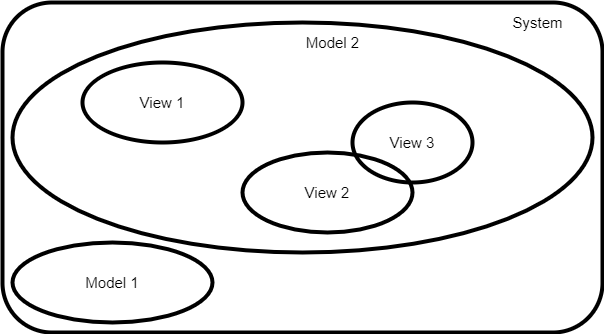
\includegraphics[scale=0.66]{Images/model_view.png}
        \caption{Rappresentazione grafica di modelli e viste nel contesto di un sistema.}
        \label{fig:model_view}
    \end{figure}
    
    \begin{figure}[h!]
        \centering
        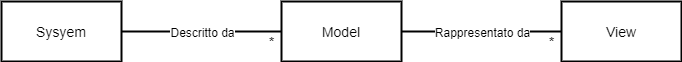
\includegraphics[width=\textwidth]{Images/model_view_UML.png}
        \caption{Un sistema può essere descritto da molti modelli, che a loro volta possono essere rappresentati da molte viste.}
        \label{fig:model_view_UML}
    \end{figure}
    
\subsection{Fenomeni e concetti}
    Un oggetto, per com'è percepito nel dominio del suo mondo, viene chiamato \textit{fenomeno}, mentre il termine \textit{concetto} può essere descritto come una tripla composta dal suo \textbf{nome}, dallo \textbf{scopo}, ossia le proprietà che un fenomeno deve avere per appartenere a quel concetto, e i \textbf{membri}, ossia i fenomeni che appartengono a quel concetto.
    
    L'\textbf{astrazione} è considerabile come l'atto di partire dai fenomeni e categorizzarli in concetti.
    
    La \textbf{modellazione} è lo sviluppo di astrazioni che rispondono a certe caratteristiche di una classe di fenomeni, ignorando le caratteristiche invece superflue.
    
\subsection{Componenti base di UML, come e quando utilizzarli}
    \begin{itemize}
        \item \textbf{Use case diagrams:} Descrivono il funzionamento del sistema dal punto di vista del cliente.
        \item \textbf{Class diagrams:} Descrive la struttura statica del sistema, solitamente composta da oggetti, attributi e relazioni fra gli stessi.
        \item \textbf{Sequence diagrams:} Descrive il comportamento dinamico del sistema, che avviene tramite lo scambio di input e output fra il sistema stesso e attori od oggetti.
        \item \textbf{Statechart diagrams:} Una macchina a stati finiti che descrive il comportamento dinamico di un singolo oggetto, delineando gli stati che può assumere e come può assumerli.
        \item \textbf{Activity diagrams:} Modella il comportamento dinamico del sistema e in particolare il workflow.
    \end{itemize}
    
    \paragraph{Diversi tipi di domini} In base al tipo di dominio in cui ci troviamo, dobbiamo assumere approcci diversi e anche il tipo di documento da produrre cambia.
    
    Nel \textbf{demonio delle applicazioni}, ossia l'ambiente in cui il sistema opera, verrà sviluppata la parte di \textbf{Requirements Analysis}, mentre nel \textbf{dominio delle soluzioni}, che riguarda le tecnologie disponibili per sviluppare il sistema, andranno sviluppate le sezioni di \textbf{System Design} e \textbf{Object Design}.
    
    \paragraph{Attori, classi, istanze} Importante è la distinzione fra questi tre concetti.
    
    Un \textbf{attore} interagisce con il sistema dall'esterno, e potrebbe essere o non essere rappresentato nello stesso.
    
    Una \textbf{classe} è invece per definizione modellata all'interno del sistema. Essa è una astrazione che modella un'entità all'interno del dominio del sistema.
    
    Infine, una \textbf{istanza} è appunto una istanziazione specifica di una classe.